\documentclass[../AbiMappe_Mathe.tex]{subfiles}

\begin{document}

\theoremstyle{nonumberplain}

\newframedtheorem{fmytheo2}{}

%qlmanage -t -s 1000 -o . picture.svg 

\section{Naive Mengenlehre}
Eine Menge ist eine Zusammenfassung von wohlbestimmten Objekten zu einem Ganzen.
Diese Objekte heissen Elemente.\\\\


\subsection{Angabe von Mengen}
\textbf{Aufzaehlung:}\\
Eine endliche Menge kann durch aufzaehlung all ihrer Elemente angegeben werde z.B. stellt\\ $M=\{1,2,3,4,5\}$, die Menge aller natuerliche Zahlen $<6$ dar.\\\\
\textbf{Bildungsgesetz:}\\
Eine unedliche Menge kann mit Hilfe eines Bildungsgesetzes angegeben werden z.B. \\$M=\{1,2,3,\dots\}=\mathbb{N}$\\\\
\textbf{Eigenschaft:}\\
Eine Teilmenge $M$ einer Menger $N$ kann mit Hilfe einer Eingenschaft $E$ die alle Elemente der Menge entweder besitzen oder nicht angegeben werden $M=\{x \in N|E(x)\}$

\subsection{Mengenbeziehungen}

\subsubsection{Elementbeziehung}
\textbf{Definition:} Sei $M$ eine beliebiege Menge dann bedeutet, $x \in M$, das wir ein beliebiges $x$ der Menge $M$ auswaehlen.

\subsubsection{Teilmenge:}
\textbf{Definition:} Sei M eine Menge. Dann heisst eine weitere Menge N Teilmenge von M wenn gilt:
\begin{align*}
x \in N \Rightarrow x \in M
\end{align*}
\textbf{Notation:} 
\begin{align*}
N \subseteq M
\end{align*}


\subsubsection{Potenzmenge}
\textbf{Defintion:} Sei $M$ eine Menge, dann nennt die Menge all ihrer Teilmengen $U$ Potenzmenge der Menge $M$.
\begin{align*}
\mathcal{P}(M) := \{U|U \subseteq M  \}
\end{align*}
\\\textbf{Beispiel:} 
\begin{align*}
\mathcal P&(\emptyset) = \{ \emptyset \}\\
\mathcal P&(\{ a \}) = \bigl\{ \emptyset, \{ a \} \bigr\}\\
\mathcal P&(\{ a, b \}) = \bigl\{ \emptyset, \{ a \}, \{ b \}, \{ a, b \} \bigr\}\\
\end{align*}

\subsubsection{Leere Menge}
\textbf{Definition:} Eine Menge $M$ die keine Elemente enhaelt nennt man leere Menge.
\begin{align*}
\emptyset:= \{\forall x:x\notin M\}  
\end{align*}\\
\textbf{Eigenschaften:}\\
\begin{description}
\vspace{-1cm}
\item[$\bullet$] ist Teilmenge jeder Menge.
\end{description}

\subsubsection{Gleichheit}
\textbf{Definition:} Seien $A,B$ Mengen, dann nennt man diese Mengen gleich wenn alle Elemente aus $A$ in $B$ und alle Elemente aus $B$ in $A$ liegen.
\begin{align*}
A = B:= A \subseteq B \land B \subseteq A =\{x|x \in A \Leftrightarrow x \in B\}
\end{align*}
\\
\subsubsection{Disjunktion(Vereinigung)}
\textbf{Definition:} Seien $N_1,N_2$ $\subseteq$ M, dann nennt man die Menge $X$ disjunktion(vereinigung) von $N_1$ und  $N_2$ wenn fuer alle $x \in X$ gilt, das $x \in N_1$ oder $x \in N_2$.
\begin{align*}
N_1 \cup N_2:=\{x \in M| x \in N_1 \lor x \in N_2 \}
\end{align*}
\\
\paragraph{Disjunktion undendlich vieler Menge}
		\hspace{0 cm} \\ \noindent \\
		Sei $\mathfrak{S}$ ein endliches oder unendliches System von Mengen, dann besteht $\underset{M \in \mathfrak{S}}{\cup}$M aus den Elementen die in mindesten einem $M \in  \mathfrak{S}$ liegen.\\\\
\textbf{Notation:}\\
\begin{align*}
\underset{k=1}{\overset{n}{\cup}}M_k \;\;bzw\;\; \underset{k=1}{\overset{\infty}{\cup}}M_k
\end{align*}\\
\textbf{Venn-Diagramm}
\begin{figure}[H]
\centering
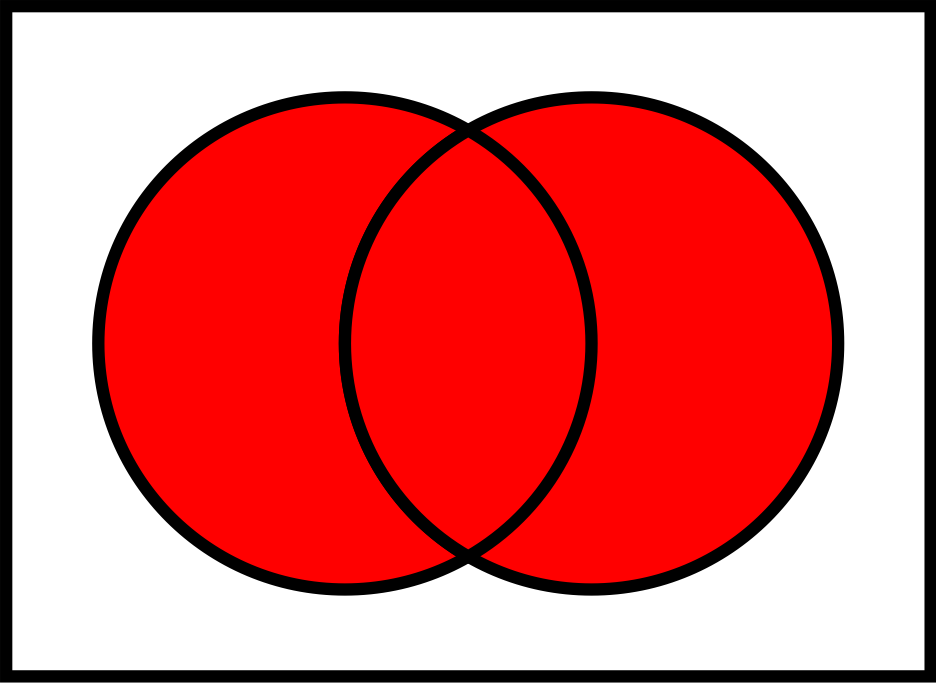
\includegraphics[width=117px, height=85.5px]{VennDis.png}
			% \captionsetup{labelformat=empty}
			% \caption{\label{fig:blue_rectangle} }
\end{figure}
\subsubsection{Konjunktion(Durchschnitt)}
\textbf{Definition:} Seien $N_1,N_2$ $\subseteq$ M, dann nennt man die Menge $X$ konjunktion(schnittmengen) von $N_1$ und  $N_2$ wenn fuer alle $x \in X$ gilt, das $x \in N_1$ und $x \in N_2$.
\begin{align*}
N_1 \cap N_2:=\{x \in M| x \in N_1 \land x \in N_2 \}
\end{align*}\\
\paragraph{Konjunktion undendlich vieler Menge}
		\hspace{0 cm} \\ \noindent \\
		Sei $\mathfrak{S}$ ein endliches oder unendliches System von Mengen, dann besteht $\underset{M \in \mathfrak{S}}{\cap}$M aus den Elementen die in jedem $M \in  $ $\mathfrak{S}$ liegen.\\\\
\textbf{Notation:}\\
\begin{align*}
\underset{k=1}{\overset{n}{\cap}}M_k \;\;bzw\;\; \underset{k=1}{\overset{\infty}{\cap}}M_k
\end{align*}\\
\textbf{Eigenschaft:}\\
\\
\begin{description}
\vspace{-1cm}
\item[$\bullet$]zwei Mengen heissen disjunkt falls $N_1$ $\cap$ $N_2$ = $\emptyset$.
\end{description}
\textbf{Venn-Diagramm}
\begin{figure}[H]
\centering
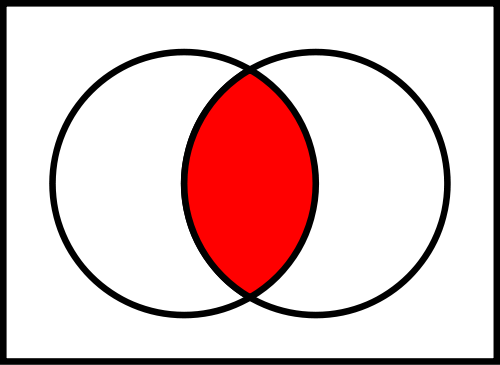
\includegraphics[width=117px, height=85.5px]{VennKon.png}
			% \captionsetup{labelformat=empty}
			% \caption{\label{fig:blue_rectangle} }
\end{figure}

\subsubsection{Komplement}
\textbf{Definition:} Sei $B$ $\subsetneq$ $M$, dann nennt man die Menge aller $x$ die in $M$ aber nicht in $B$ sind komplement von $B$ im Bezug auf $M$. Es wird mit $B^c$ notiert.
\begin{align*}
B^c:=\{x|x \notin B\}
\end{align*}
\\
\textbf{Venn-Diagramm}
\begin{figure}[H]
\centering
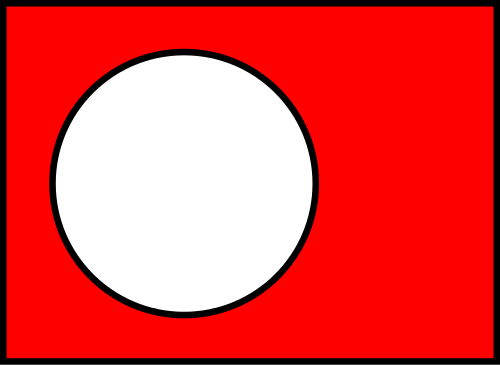
\includegraphics[width=117px, height=85.5px]{VennKom.png}
			% \captionsetup{labelformat=empty}
			% \caption{\label{fig:blue_rectangle} }
\end{figure}


\subsubsection{Differenz}
\textbf{Definition:} Seien $A,B$ Mengen, dann nennt man alle $x$ die in $A$ aber nicht in $B$ sind Differenz von $A$ und $B$.
\begin{align*}
A \setminus B:=\{x|x \in A \land x \notin B\}
\end{align*}
\\
\textbf{Venn-Diagramm}
\begin{figure}[H]
\centering
\includegraphics[width=117px, height=85.5px]{VennDiff.png}
			% \captionsetup{labelformat=empty}
			% \caption{\label{fig:blue_rectangle} }
\end{figure}

A=B
Hat man eine solche Gleichung zu beweisen, so muß man also zeigen, daß aus x $\in$ M stets x $\in$ N und umgekehrt aus x $\in$ N auch immer x $\in$ M folgt. bzw M $\subseteq$ N und umgekehrt
 $\mathfrak{S}$

 \section{Beweise}
 \subsection{Morganschen Komplementierungsregeln}
 Sind alle Mengen M $\in \mathfrak{S}$ Teilmengen einer festen Universalmenge U und bezeichnen wir das Komplement U ohne N einer Teilmenge N von U der Kürze halber mit $N^c$.\\\\
 \textbf{1. }Das Komplement der Vereinigung ist gleich dem Durchschnitt der Komplemente.\\
 \begin{align*}
	(\underset{M \in \mathfrak{S}}{\overset{}{\cup}}M)^c =  \underset{M \in \mathfrak{S}}{\overset{}{\cap}}(M^c)
 \end{align*}
 Da klar is das M $\in \mathfrak{S}$ wird dies beim folgenden Beweis nicht weiter angegeben.\\
\textbf{Beweis:}\\\\
\textbf{A $\Rightarrow$ B }
\begin{align*}
	x \in (\cup M)^c \Rightarrow (x \in U \land x \notin \cup M ) \Rightarrow (x \in U \land x \notin \cup M \; \forall \; M \in \mathfrak{S}) \Rightarrow x\in M^c\;\forall\; M \Rightarrow x \in \cap(M^c)\\
	\blacksquare
 \end{align*}
 \textbf{B $\Rightarrow$ A }\\
 \begin{align*}
 x \in \cap (M^c) \Rightarrow (x \in M^c\;\forall\;M^c) \Rightarrow (x \in U \land x \notin M\; \forall\; M) \Rightarrow (x \in U \land x \notin \cup M) \Rightarrow x \in (\cup M)^c\\
 \blacksquare
 \end{align*}
 \textbf{A $\Leftrightarrow$ B}
 \\\textbf{2. }Das Komplement des Durchschnitts ist gleich der Vereinigung der Komplemente.\\
 \begin{align*}
	(\underset{M \in \mathfrak{S}}{\overset{}{\cap}}M)^c =  \underset{M \in \mathfrak{S}}{\overset{}{\cup}}(M^c)
 \end{align*}
\textbf{Beweis:}\\\\
\textbf{A $\Rightarrow$ B } 
\begin{align*}
x \in (\cap M)^c \Rightarrow (x \in U \land x \notin \cap M) \Rightarrow (x \in U \land \exists M : x \notin M ) \Rightarrow (\exists M : x \in M^c ) \Rightarrow (x \in \cup (M^c))\\
 	\blacksquare
% x \in (\cap M)^c \Rightarrow (x \in U \land x \in \cap M^c \;\exists M)
\end{align*}
 \textbf{B $\Rightarrow$ A }\\
 \begin{align*}
 x \in \cup(M^c) \Rightarrow (x \in U \land \exists M : x \in M^c ) \Rightarrow (\exists M : x \notin M) \Rightarrow ( x \notin \cap M) \Rightarrow (x \in (\cap M)^c)\\
 	\blacksquare
 \end{align*}



\end{document}